\documentclass[aspectratio=169,10pt]{beamer}

% metropolis without its font theme (that one needs XeLaTeX for the Fira fonts)
\useinnertheme{metropolis}
\useoutertheme[progressbar=frametitle,numbering=fraction]{metropolis}
\usecolortheme{metropolis}
\usepackage{amsmath}
\usepackage{txfonts}  % Times math, close to the STIX fonts in the figures
\usefonttheme[onlymath]{serif}
\usepackage{booktabs}
\usepackage{animate}
\usepackage{appendixnumberbeamer}

\graphicspath{{../figures/}}
\pdfstringdefDisableCommands{\def\translate#1{#1}}  % lets \appendix make its bookmark
\setbeamerfont{footnote}{size=\tiny}
\setbeamerfont{title}{size=\Large}
\setbeamerfont{subtitle}{size=\normalsize}
\setbeamertemplate{caption}{\insertcaption}

\newcommand{\avg}[1]{\langle #1 \rangle}
\newcommand{\ee}{\mathrm{e}}
\newcommand{\src}[1]{{\small\color{gray}[#1]}}

\title{Dynamical Localization in the Quantum Kicked Rotor}
\subtitle{How quantum mechanics stops chaotic diffusion}
\author{Wei Chen}
\institute{PHY-315 Quantum Mechanics, final project}
\date{November 2026}

\begin{document}

% metropolis stacks a page-high box on the title page; the slide is fine, so don't report it
{\vfuzz=20pt\maketitle}

% ---------------------------------------------------------------------------
\begin{frame}{The question}
  \begin{itemize}
    \item Classical chaos: nearby orbits separate like $\ee^{\lambda t}$, and a chaotic system can spread forever
    (diffusion).
    \item Quantum mechanics: the Schr\"odinger equation is \alert{linear and unitary}. Nothing separates
    exponentially.
    \item So what does a quantum system do when its classical version is chaotic?
  \end{itemize}
  \vspace{0.6em}
  \textbf{The simplest test case: the kicked rotor.}
  \begin{itemize}
    \item Classically, strong kicks make the momentum perform a random walk: the energy grows linearly forever.
    \item Quantum mechanically, the growth follows the classical one for a while, then \alert{stops}.
    \item This is \alert{dynamical localization}. It is closely related to Anderson localization, and it was
    seen with cold atoms in 1995.
  \end{itemize}
\end{frame}

% ---------------------------------------------------------------------------
\begin{frame}{The kicked rotor}
  A particle on a ring, kicked once per period with a strength that depends on its angle:
  \[
    H = \frac{p^2}{2} + K\cos\theta\sum_{n}\delta(t - n)
  \]
  Integrating Hamilton's equations over one period gives the \alert{standard map}:
  \[
    p_{n+1} = p_n + K\sin\theta_n, \qquad \theta_{n+1} = \theta_n + p_{n+1} \pmod{2\pi}
  \]
  \begin{itemize}
    \item $K$: kick strength, controls the chaos.
    \item The momentum is never wrapped: its growth is what we measure.
    \item Quantum version: $p = \hbar m$ with integer $m$; $\hbar$ is the effective Planck constant
    ($\hbar\to0$ is the classical limit).
    \item Matched starting points: quantum state $m = 0$; classical ensemble $p = 0$, $\theta$ uniform.
  \end{itemize}
\end{frame}

% ---------------------------------------------------------------------------
\begin{frame}{Classical dynamics: from order to chaos}
  \begin{columns}[T,onlytextwidth]
    \begin{column}{0.47\textwidth}
      \centering
      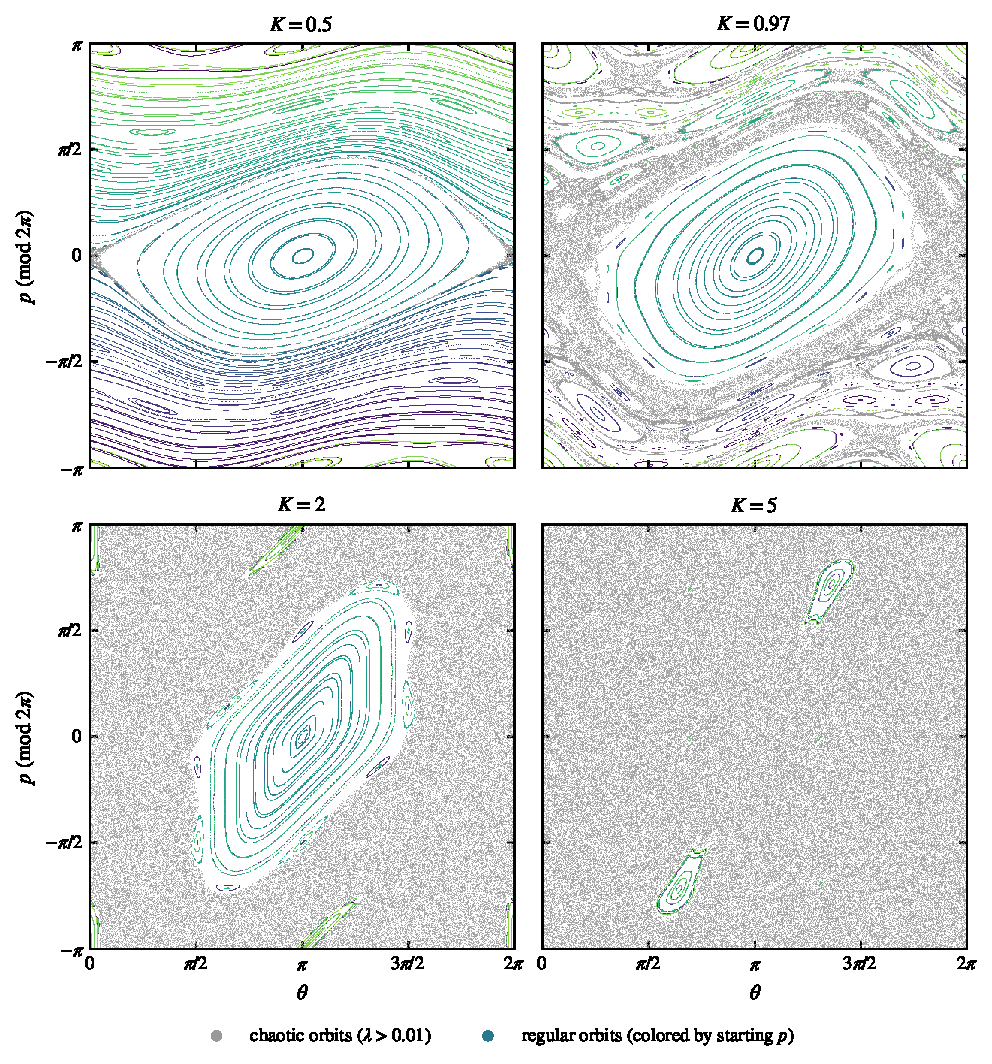
\includegraphics[width=\linewidth,height=0.8\textheight,keepaspectratio]{01_phase_portraits.pdf}
    \end{column}
    \begin{column}{0.5\textwidth}
      \begin{itemize}
        \item Gray: chaotic orbits ($\lambda > 0.01$). Colors: regular orbits.
        \item Weak kicks: invariant curves act as walls in momentum.
        \item The last wall breaks at $K_c = 0.9716$ \src{Greene 1979}.
        \item Chaotic area: 1\%, 43\%, 76\%, 98\% at $K = 0.5$, 0.97, 2, 5.
        \item At $K = 5$: $\lambda = 0.98$, close to Chirikov's $\ln(K/2) = 0.92$ \src{Chirikov 1979}.
      \end{itemize}
    \end{column}
  \end{columns}
\end{frame}

% ---------------------------------------------------------------------------
\begin{frame}{Classical diffusion and its Bessel corrections}
  \begin{columns}[T,onlytextwidth]
    \begin{column}{0.5\textwidth}
      \centering
      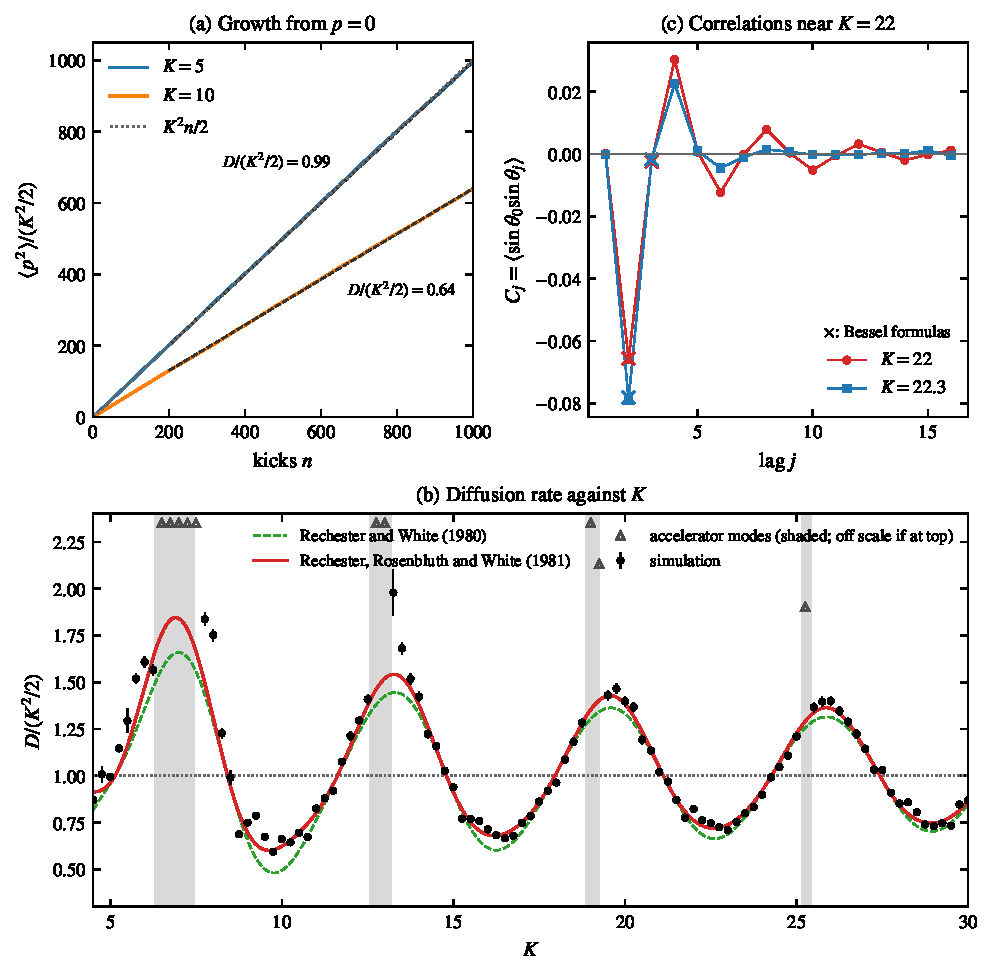
\includegraphics[width=\linewidth,height=0.8\textheight,keepaspectratio]{02_classical_diffusion.pdf}
    \end{column}
    \begin{column}{0.48\textwidth}
      \small
      \begin{itemize}
        \item Random phases give $\avg{p^2} \approx Dn$ with $D = K^2/2$.
        \item Correlations $C_j = \avg{\sin\theta_0\sin\theta_j}$ correct it:
        \[ \frac{D}{K^2/2} \approx 1 - 2J_2 - 2J_1^2 + 2J_3^2 + 2J_2^2 \]
        \src{Rechester \& White 1980; Rechester, Rosenbluth \& White 1981}
        \item Measured: $D/(K^2/2) = 0.995 \pm 0.009$ at $K = 5$, $0.638 \pm 0.006$ at $K = 10$.
        \item Shaded: accelerator modes, where orbits fly ballistically.
        \item Remaining misses come from long correlations ($C_4$ at $K = 22$).
      \end{itemize}
    \end{column}
  \end{columns}
\end{frame}

% ---------------------------------------------------------------------------
\begin{frame}{The quantum rotor: one period at a time}
  The kick is instantaneous, so one period is exactly a kick followed by free rotation:
  \[
    \hat U = \ee^{-i\hat p^2/2\hbar}\,\ee^{-iK\cos\hat\theta/\hbar},
    \qquad
    \langle m'|\hat U|m\rangle = \ee^{-i\hbar m'^2/2}\,(-i)^{m'-m}\,J_{m'-m}(K/\hbar)
  \]
  \begin{itemize}
    \item One kick couples each momentum state to about $k = K/\hbar$ neighbors.
    \item Two parameters: $K$ (classical chaos) and $\hbar$ (how quantum).
  \end{itemize}
  \textbf{Numerics:} store $\psi$ on $N$ angles; per period
  \begin{enumerate}
    \item multiply by $\ee^{-iK\cos\theta/\hbar}$, \quad 2. FFT to momentum, \quad 3. multiply by
    $\ee^{-i\hbar m^2/2}$, \quad 4. inverse FFT.
  \end{enumerate}
  \begin{itemize}
    \item Exact, not an approximation (kick and free step act at different times). Only the momentum range and
    roundoff limit it.
    \item $N = 2^{14}$ states; probability near the grid edge kept below $10^{-10}$. About 1 ms per kick.
  \end{itemize}
\end{frame}

% ---------------------------------------------------------------------------
\begin{frame}{Validation: five checks, 39 tests}
  \small
  \begin{tabular}{@{}lp{0.40\textwidth}p{0.37\textwidth}@{}}
    \toprule
    Check & Test & Result \\
    \midrule
    1. Norm & $\avg{\psi|\psi} = 1$ over 1000 kicks & drift $3\times10^{-16}$ per kick \\
    2. Resonance & $\hbar = 4\pi$: $\avg{p^2} = K^2n^2/2$; $\hbar = 2\pi$: return after 2 kicks &
      errors $\le 3\times10^{-13}$ \\
    3. Early times & exact $\avg{p^2}$ after 1 and 2 kicks; $\hbar^2$ convergence at 3 kicks &
      $10^{-15}$; observed order 1.97 \\
    4. Grid & $N = 2^{14}$ vs $2^{15}$; edge probability & edge $3\times10^{-27}$; $2^{12}$ fails \\
    5. Time reversal & $n$ kicks forward, $n$ back & quantum $3\times10^{-13}$ after 1000; classical fails at 38 \\
    \bottomrule
  \end{tabular}
  \vspace{0.8em}
  \begin{itemize}
    \item Every tolerance has a stated reason: machine precision, statistical error, or known physics.
    \item Testing the tests: six planted bugs, each caught by at least one test.
  \end{itemize}
\end{frame}

% ---------------------------------------------------------------------------
\begin{frame}{An exact test: quantum resonance}
  \begin{columns}[T,onlytextwidth]
    \begin{column}{0.5\textwidth}
      \centering
      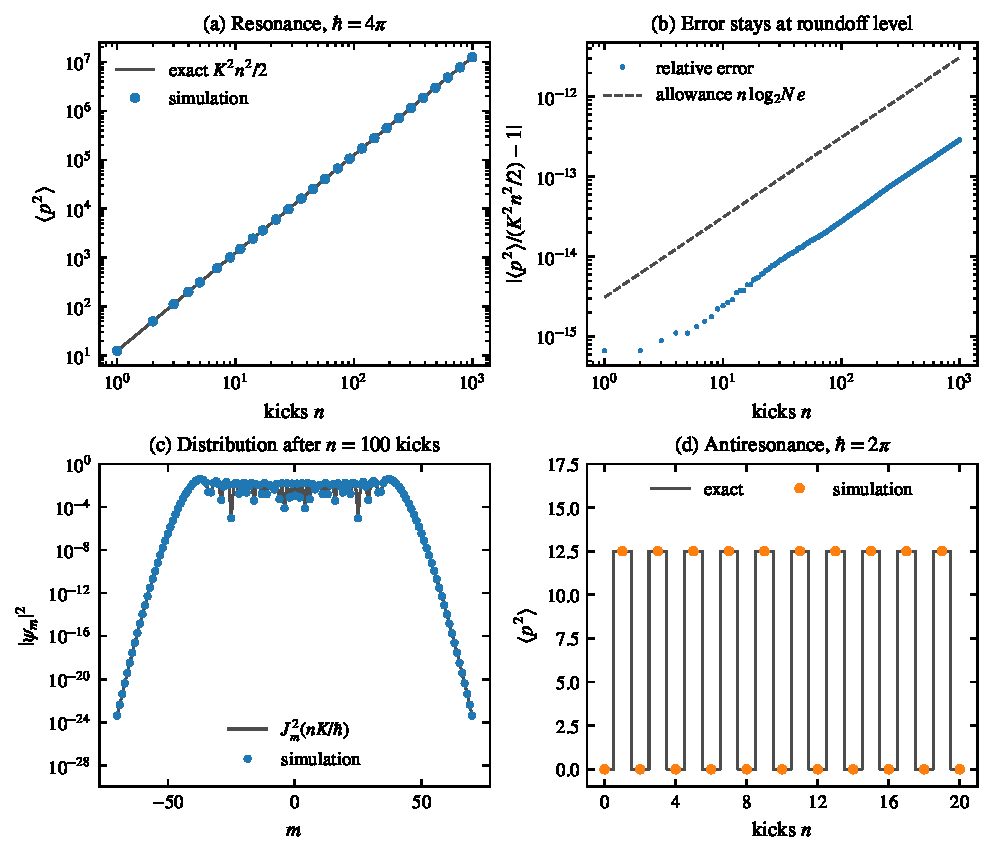
\includegraphics[width=\linewidth,height=0.8\textheight,keepaspectratio]{05_resonance_test.pdf}
    \end{column}
    \begin{column}{0.48\textwidth}
      \begin{itemize}
        \item $\hbar = 4\pi$: $\ee^{-i\hbar m^2/2} = 1$, so the kicks add up coherently:
        \[ |\psi_m|^2 = J_m^2(nK/\hbar), \]
        \[ \avg{p^2} = \tfrac12 K^2n^2 \]
        Ballistic, faster than diffusion \src{Casati et al.\ 1979}.
        \item $\hbar = 2\pi$: free step shifts $\theta$ by $\pi$, the next kick cancels: exact return every
        2 kicks (``antiresonance'').
        \item The code reproduces both to $\sim10^{-13}$.
      \end{itemize}
    \end{column}
  \end{columns}
\end{frame}

% ---------------------------------------------------------------------------
\begin{frame}{Main result: the quantum growth stops}
  \centering
  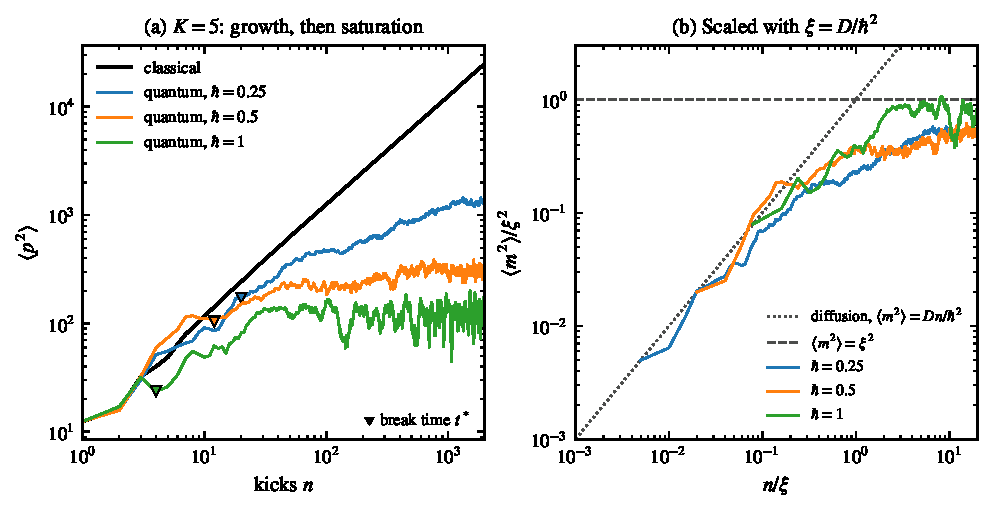
\includegraphics[height=0.62\textheight]{03_quantum_vs_classical.pdf}
  \begin{itemize}
    \small
    \item Classical: $D = 12.51 \pm 0.10$, grows forever. Quantum ($K = 5$): follows, then saturates.
    \item Break times (25\% below classical): 20, 12, 4 kicks at $\hbar = 0.25$, 0.5, 1. Right: rescaled
    with $\xi = D/\hbar^2$.
  \end{itemize}
\end{frame}

% ---------------------------------------------------------------------------
\begin{frame}{Why it stops: Floquet theory}
  Eigenstates of the one-period operator: $\hat U|\phi_k\rangle = \ee^{-i\omega_k}|\phi_k\rangle$
  (quasienergies $\omega_k$). Then
  \[
    \avg{p^2}_n = \sum_{k,k'} c_k^*c_{k'}\,\ee^{in(\omega_k - \omega_{k'})}\,\langle\phi_k|\hat p^2|\phi_{k'}\rangle
  \]
  \begin{itemize}
    \item If the $|\phi_k\rangle$ are \alert{localized} in momentum, only finitely many terms matter: the energy
    is quasi-periodic and bounded.
  \end{itemize}
  \textbf{How long until it stops?}
  \begin{itemize}
    \item About $\xi$ states involved, quasienergy spacing $\sim 2\pi/\xi$, resolved after $t^* \sim \xi$ kicks.
    \item Until then it diffuses: $\avg{m^2} \approx Dt/\hbar^2$. Consistency: $\xi^2 \sim D\xi/\hbar^2$, so
    \[
      \xi \sim \frac{D}{\hbar^2}, \qquad t^* \sim \frac{D}{\hbar^2}, \qquad \avg{p^2}_\infty \sim \frac{D^2}{\hbar^2}
    \]
    \item The limits $\hbar\to0$ and $n\to\infty$ do not commute.
  \end{itemize}
\end{frame}

% ---------------------------------------------------------------------------
\begin{frame}{Watching it happen}
  \centering
  \animategraphics[height=0.6\textheight,controls,loop,autoplay,poster=last]{12}{anim/frame_}{000}{078}

  \small Momentum distribution, $K = 5$, $\hbar = 0.25$, up to 1000 kicks (frames speed up). Red: classical
  keeps widening. Blue: quantum stops.

  \tiny (The animation plays in Adobe Acrobat Reader, other viewers show the last frame; the file \texttt{figures/04\_momentum\_distribution.gif}
  plays anywhere.)
\end{frame}

% ---------------------------------------------------------------------------
\begin{frame}{The localized momentum distribution}
  \centering
  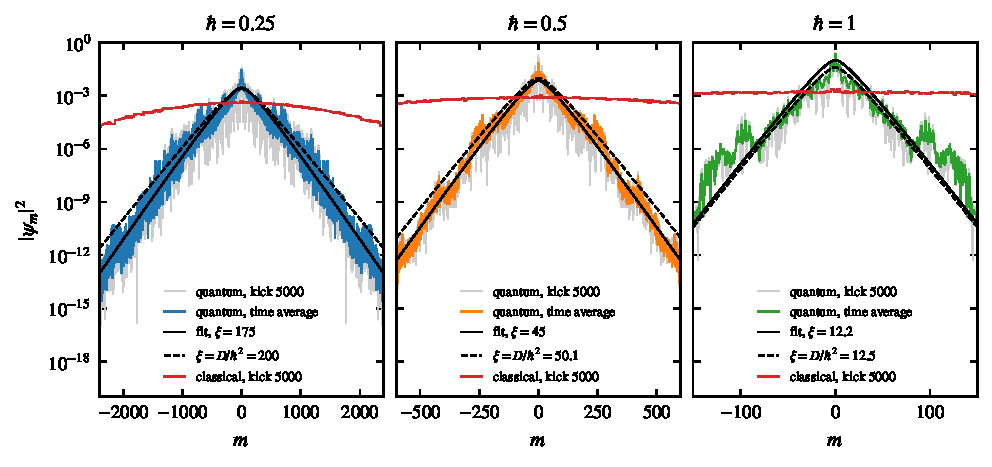
\includegraphics[width=0.86\textwidth]{04_momentum_distribution.pdf}
  \begin{itemize}
    \small
    \item Exponential tails over 13 decades. Izrailev's shape \src{Izrailev 1990}:
    $\overline{P}(m) = \frac{1}{2\xi}\bigl(1 + \frac{2|m|}{\xi}\bigr)\ee^{-2|m|/\xi}$
    \item Fitted $\xi/(D/\hbar^2) = 0.87$, 0.90, 0.98; earlier work: $1.04 \pm 0.20$ \src{Shepelyansky 1986}.
  \end{itemize}
\end{frame}

% ---------------------------------------------------------------------------
\begin{frame}{How the localization length scales}
  \begin{columns}[T,onlytextwidth]
    \begin{column}{0.62\textwidth}
      \centering
      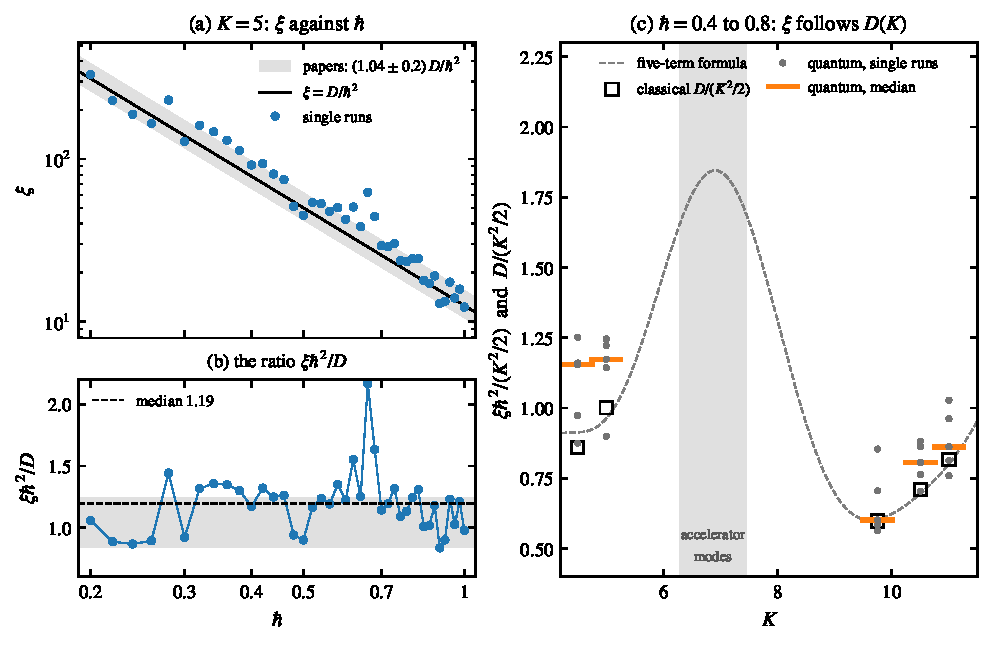
\includegraphics[width=\textwidth]{07_bonus_xi_scaling.pdf}
    \end{column}
    \begin{column}{0.36\textwidth}
      \small
      \begin{itemize}
        \item 41 values of $\hbar$ at $K = 5$: $\xi$ follows $D/\hbar^2$ over a factor 27.
        \item $\xi\hbar^2/D$: median 1.19, spread 0.25; it wanders in bands (cause unknown).
        \item Varying $K$: $\xi$ follows the classical $D(K)$, including its Bessel dip at $K \approx 9.75$,
        not $K^2/2$.
        \item Near a rational $\hbar/4\pi$ localization can fail: $0.714/4\pi$ is $1.4\times10^{-7}$ from
        $5/88$.
      \end{itemize}
    \end{column}
  \end{columns}
\end{frame}

% ---------------------------------------------------------------------------
\begin{frame}{Why the states localize: the Anderson analogy}
  Fishman, Grempel and Prange \src{1982}: write the kick as $\ee^{-ik\cos\theta} = \frac{1 + iW}{1 - iW}$,
  $W = -\tan\frac{k\cos\theta}{2}$. The Floquet equation becomes
  \[
    T_m v_m + \sum_{r\neq0} W_r\,v_{m+r} = -W_0\,v_m,
    \qquad T_m = \tan\Bigl(\frac{\omega - \hbar m^2/2}{2}\Bigr)
  \]
  \begin{itemize}
    \item A particle hopping on a 1D lattice of momentum states, with on-site energies $T_m$.
    \item $\hbar/4\pi$ irrational: $\hbar m^2/2 \bmod 2\pi$ looks random, $T_m$ is Cauchy distributed:
    the \alert{Lloyd model}, all states localized.
    \item $\hbar/4\pi$ rational: $T_m$ periodic, Bloch waves, unbounded growth (resonance).
    \item Time-periodic kicking plays the role of static disorder.
  \end{itemize}
\end{frame}

% ---------------------------------------------------------------------------
\begin{frame}{Early times: how long does quantum follow classical?}
  After one kick both give $K^2/2$ exactly. After two kicks:
  \[
    \avg{p^2}_2^{\rm qm} = K^2\Bigl[1 + \cos\tfrac{\hbar}{2}\bigl(J_0(K_q) - J_2(K_q)\bigr) - \tfrac12 J_2(K_2)\Bigr],
    \quad K_q = \tfrac{2K}{\hbar}\sin\tfrac{\hbar}{2},\ K_2 = \tfrac{2K}{\hbar}\sin\hbar
  \]
  \begin{itemize}
    \item $\hbar\to0$ gives the classical formula; the gap is $O(\hbar^2)$: 1.0\% at $\hbar = 0.25$.
    \item The $\hbar^2$ coefficient explodes: $-0.2$, $-35$, $-550$ at $n = 2$, 3, 4.
    \item Chaos magnifies quantum effects by $\ee^{\lambda}$ per kick: detailed agreement only until the
    \alert{Ehrenfest time} $t_E \sim \lambda^{-1}\ln(1/\hbar)$, a few kicks.
    \item After that only statistics survive (the diffusion rate), until the break time $t^* \sim D/\hbar^2$.
  \end{itemize}
\end{frame}

% ---------------------------------------------------------------------------
\begin{frame}{Time reversal: chaos against unitarity}
  \begin{columns}[T,onlytextwidth]
    \begin{column}{0.58\textwidth}
      \centering
      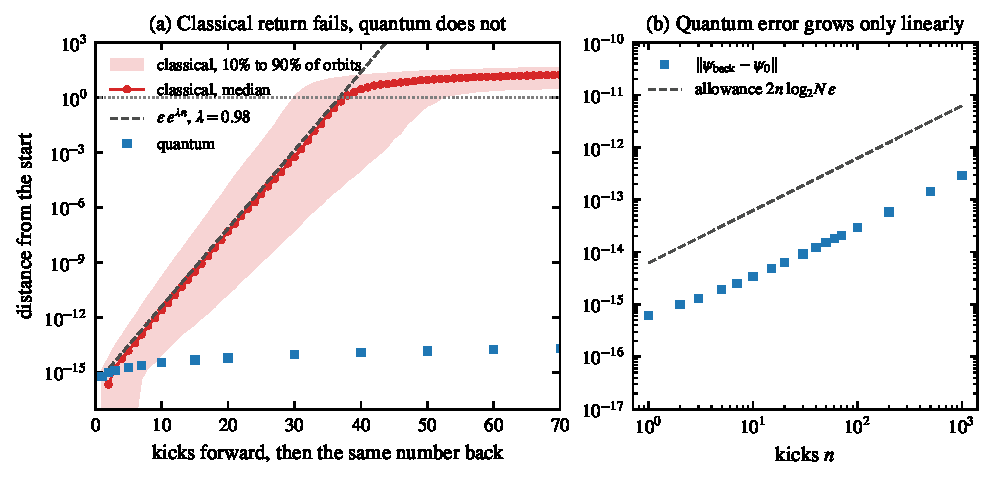
\includegraphics[width=\textwidth]{06_time_reversal.pdf}
    \end{column}
    \begin{column}{0.4\textwidth}
      \small
      \begin{itemize}
        \item Run $n$ kicks forward, $n$ back.
        \item Classical: roundoff grows like $\varepsilon\,\ee^{\lambda n}$; fails at $n = 38$ (predicted 36.7).
        \item Quantum: $\|\hat U(\psi + \delta) - \hat U\psi\| = \|\delta\|$, so errors only add up:
        $3\times10^{-13}$ after 1000 kicks.
        \item Bonus: the same code on Windows and Linux gives identical quantum numbers, but different
        classical orbits (statistics agree).
      \end{itemize}
    \end{column}
  \end{columns}
\end{frame}

% ---------------------------------------------------------------------------
\begin{frame}{Three time scales}
  \begin{center}
  \begin{tabular}{@{}llll@{}}
    \toprule
    Time & Scale & What holds & $\hbar = 0.25$, $K = 5$ \\
    \midrule
    Ehrenfest time & $t_E \sim \lambda^{-1}\ln(1/\hbar)$ & detailed correspondence & about 1 kick \\
    Break time & $t^* \sim D/\hbar^2$ & classical diffusion rate & 20 kicks (25\% rule) \\
    Saturation & a few $\xi$ & localized, quasi-periodic & a few hundred kicks \\
    \bottomrule
  \end{tabular}
  \end{center}
  \vspace{0.6em}
  \begin{itemize}
    \item As $\hbar\to0$ at fixed $n$, both times go to infinity: the classical limit is recovered.
    \item At any fixed $\hbar$, the long-time behavior is fundamentally quantum.
    \item The saturated energy still swings slowly (17\% rms over 40000 kicks): beats between quasienergies.
  \end{itemize}
\end{frame}

% ---------------------------------------------------------------------------
\begin{frame}{In the lab: cold atoms}
  Moore, Robinson, Bharucha, Sundaram and Raizen \src{1995}:
  \begin{itemize}
    \item Ultracold sodium atoms in a pulsed standing wave of light: potential $\propto \cos(2k_L x)$,
    so $\theta = 2k_Lx$; momentum in units of $2\hbar k_L$.
    \item Kick strength $\kappa = 11.6$, scaled Planck constant $\bar k = 8\omega_rT = 2.0$.
    \item Diffusion at the classical rate $\kappa^2/2$, break after about 8 kicks, then exponentially
    localized (checked to 50 kicks).
    \item Their $\xi = \kappa^2/4\bar k^2 \approx 8.3$ is the $1/e$ point of the probability: half of our
    $\xi = D/\hbar^2$.
    \item They also saw the resonances, and the antiresonance sign flip in the first kicks.
  \end{itemize}
\end{frame}

% ---------------------------------------------------------------------------
\begin{frame}{Conclusions}
  \begin{itemize}
    \item Classical: diffusion with $D(K)$ oscillating around $K^2/2$; the Bessel expansion works to
    about 4\%.
    \item Quantum: follows the classical growth up to $t^* \sim D/\hbar^2$, then stops.
    \item Momentum distribution: exponentially localized, $\xi \approx 1.2\,D/\hbar^2$ ($\pm20\%$), following
    $D(K)$.
    \item Floquet theory explains the saturation; the Anderson mapping explains the localization.
    \item Unitarity versus chaos: quantum errors never grow exponentially.
  \end{itemize}
  \textbf{Open questions from this project}
  \begin{itemize}
    \item Why does $\xi\hbar^2/D$ wander in bands as $\hbar$ changes?
    \item What causes the narrow central peak of the averaged distribution?
  \end{itemize}
\end{frame}

% ---------------------------------------------------------------------------
\begin{frame}{References}
  \scriptsize
  \begin{itemize}
    \item G. Casati, B. V. Chirikov, F. M. Izraelev, J. Ford, in \emph{Stochastic Behavior in Classical and
    Quantum Hamiltonian Systems}, Lect.\ Notes Phys.\ \textbf{93}, 334 (1979).
    \item B. V. Chirikov, Phys.\ Rep.\ \textbf{52}, 263 (1979).
    \item J. M. Greene, J. Math.\ Phys.\ \textbf{20}, 1183 (1979).
    \item A. B. Rechester and R. B. White, Phys.\ Rev.\ Lett.\ \textbf{44}, 1586 (1980).
    \item A. B. Rechester, M. N. Rosenbluth, R. B. White, Phys.\ Rev.\ A \textbf{23}, 2664 (1981).
    \item F. M. Izrailev and D. L. Shepelyansky, Theor.\ Math.\ Phys.\ \textbf{43}, 553 (1980).
    \item S. Fishman, D. R. Grempel, R. E. Prange, Phys.\ Rev.\ Lett.\ \textbf{49}, 509 (1982).
    \item D. L. Shepelyansky, Phys.\ Rev.\ Lett.\ \textbf{56}, 677 (1986).
    \item F. M. Izrailev, Phys.\ Rep.\ \textbf{196}, 299 (1990).
    \item F. L. Moore, J. C. Robinson, C. F. Bharucha, B. Sundaram, M. G. Raizen, Phys.\ Rev.\ Lett.\
    \textbf{75}, 4598 (1995).
    \item F. Saif, Phys.\ Rep.\ \textbf{419}, 207 (2005).
  \end{itemize}
\end{frame}

% ---------------------------------------------------------------------------
\appendix

\begin{frame}{Backup: where the Bessel corrections come from}
  \small
  $D = K^2\bigl[C_0 + 2\sum_{j\ge1}C_j\bigr]$ with $C_j = \avg{\sin\theta_0\sin\theta_j}$ over the torus.
  \begin{itemize}
    \item $(\theta_0, \theta_1)$ are independent and uniform (the change of variables from $(\theta_0, p_0)$ is
    a shear), and $\theta_{j+1} = 2\theta_j - \theta_{j-1} + K\sin\theta_j$.
    \item Expand with $\ee^{iz\sin\theta} = \sum_l J_l(z)\ee^{il\theta}$ and keep the terms in which all
    angles cancel:
    \[
      C_0 = \tfrac12,\quad C_1 = 0,\quad C_2 = -\tfrac12 J_2(K),\quad C_3 = \tfrac12\bigl[J_3^2(K) - J_1^2(K)\bigr]
    \]
    \item Lags up to 3 give $D/(K^2/2) = 1 - 2J_2 - 2J_1^2 + 2J_3^2$; the next order adds $2J_2^2$.
    \item Checked at $K = 22$: $C_2 = -0.0658$ (formula $-0.0657$), $C_3 = -0.0024$ ($-0.0025$).
  \end{itemize}
\end{frame}

\begin{frame}{Backup: the quantum two-kick result}
  \small
  Heisenberg picture with $\hat U = F\hat K$: $p_2 = \hat p + K\sin\theta_0 + K\sin\theta_1$, and $\hat p|0\rangle = 0$.
  \begin{itemize}
    \item Through one free step the kick is weakened:
    \[
      \hat U^\dagger\ee^{in\theta}\hat U = \ee^{i\hbar n^2/2}\,\ee^{in\theta}\,\ee^{iK_n\sin(\theta + n\hbar/2)}\,T^n,
      \qquad K_n = \frac{2K}{\hbar}\sin\frac{n\hbar}{2}
    \]
    with $T$ the shift of $\theta$ by $\hbar$.
    \item $\avg{\sin^2\theta_1} = \frac12[1 - J_2(K_2)]$ and
    $\avg{\{\sin\theta_0,\sin\theta_1\}} = \cos\frac{\hbar}{2}\,[J_0(K_q) - J_2(K_q)]$.
    \item Limits: $\hbar\to0$ classical; $\hbar = 4\pi$ gives $2K^2$ (resonance); $\hbar = 2\pi$ gives 0
    (antiresonance).
    \item The FFT code reproduces it to $10^{-15}$.
  \end{itemize}
\end{frame}

\begin{frame}{Backup: when the classical \texorpdfstring{$D$}{D} is ambiguous}
  \begin{itemize}
    \item $K = 9.25$: the line $p = 0$ crosses an island that traps 9\% of the matched ensemble forever.
    \item Matched ensemble: $D/(K^2/2) = 0.718$. Uniform torus ensemble: $0.800$. Both steady over 4000 kicks.
    \item Near the accelerator windows ($6.28 \le K \le 7.45$ for $l = 1$) diffusion is anomalous: at
    $K = 5.5$ the kurtosis of $\Delta p$ is about 300.
    \item So experiment 07 uses $K = 4.5$, 5, 9.75, 10.5 and 11, where both ensembles agree.
  \end{itemize}
\end{frame}

\end{document}
